\section{Executive Summary}

\parskip0pt Understanding the formation and evolution of galaxies is
one of the foremost goals of astrophysics and cosmology
today.
The cosmic star formation rate has undergone a dramatic evolution of the course of the last seven billion years.  Dust-obscured star forming galaxies (DSFGs) offer the perfect tracers of this evolution as they contain much of the star-forming activity.
By their very nature, DSFGs are difficult to study and have, until recently, been poorly understood.
A variety of unextincted diagnostic lines are present in the far-infrared
(FIR) which can provide insight into the conditions of star
formation, including the instantaneous star formation rate, the effect of AGN feedback on star formation, the mass function of the stars, and the spectrum of their ionizing radiation.

Spectroscopy in the far-infrared is technically difficult but scientifically crucial, as underscored by the Decadal Review's endorsement of US involvement in the Japanese-led Space Infrared Telescope for Cosmology and Astrophysics (SPICA), a 4 K, 3 meter telescope optimized for FIR spectroscopy.  Involvement at the level of a complete NASA-funded instrument now seems unlikely in the current budgetary environment (though small critical hardware contributions are under consideration).  FIR spectroscopy from space-based platform with a cryogenic mirror can, in principle, achieve performance limited by astrophysical backgrounds.  However, we argue that stratospheric balloons offer a platform which can outperform current capabilities and are competitive against satellite missions for large area, spatial/spectral mapping. 
This is possible for a telescope using low-emissivity, high-throughput optics onto a dispersive spectrometer, and having high-sensitivity, large-format detector arrays.

We propose an aggressive program of instrumentation development and experimental study called the \namefull\ (\name), with the goal of demonstrating the key technical milestones necessary for balloon-borne FIR spectroscopy limited by the photon noise from the atmosphere. \name\ will address the two key technical issues necessary to achieve this:
\begin{enumerate}
\parskip-5pt
\item	Low emissivity, high throughput telescope and spectrometer optics 
\item	Background limited detectors in large format arrays, scalable to $>10^4$ pixels
\end{enumerate}
\parskip-5pt
We will do this by constructing an integral-field spectrometer from 240 - 420
\mum\ coupled to a \D\ off-axis telescope.  For the detectors, we will leverage the highly advanced development work of Jonas Zmuidzinas' group at Caltech / JPL on kinetic inductance detectors (KIDs).  KIDs represent the most promising route to economical, large format submillimeter detector arrays.  In addition to this technical demonstration, we will be able to obtain scientific results from \name\ from two North American overnight flights which will
\parskip-5pt
\begin{enumerate}
\parskip-5pt

\item \label{goal:Lines} Obtain spectra of $\sim100$ galaxies in the fine structure lines \cii(157 \mum) ($0.5 < z < 1.54$), and for lensed galaxies, \oi(63 \mum), and \oiii(88 \mum) ($2 < z < 4$)

\item \label{goal:PowerSpectrum} Demonstrate deep tomographic maps capable of detecting the shot noise power spectrum of \cii\ at $z\sim1$

\end{enumerate}
\parskip-5pt
With these goals met, it is our explicit intention to build upon this proposal in order to successfully propose a wholly unprecedented experiment to study the cosmic star formation history.  This future experiment will make a 3-D cube spanning spanning at once at least 4 billion years of
cosmic history ($0.5 < z < 1.5$), on scales from 1 - 50 Mpc (30\arcsec\ to $>1\arcdeg$) with complete spectroscopic
information.   This would be done with fully three dimensional tomographic maps
of emission in \cii\ and other lines.
Such an experiment fills a unique and vital scientific niche not filled by \herschel, SOFIA, ALMA, or even SPICA.

% from the unobscured ionized carbon fine structure line
% \cii(157.7 \mum,) 
% The total cost for a
% 5-year program to build, fly, and analyze the data from \icaris\ was \$6.84M.  
% Though this proposal was very highly ranked, it was not funded.  

% 
% 
% 
% \name\ will retain the telescope aperture (2.5 meter) and total spectral coverage (240 - 420 \mum) as \icaris, but we have reduced costs by reducing the flight program to two North American flights (instead of an LDB flight), and reducing the instantaneous spectral coverage to half (with the full range covered by scanning the diffraction grating). 
\parskip0pt


%can be extended to LDB with longer hold-time cryostat 




%In addition, we will characterize the atmospheric emissivity beyond the purely %theoretical models currently available.  


We stress that much of the work for \name, including the telescope and spectrometer optics, detectors, and detector readout, can be directly re-used in a future experiment. The frequency domain RF readout of KIDs is relatively inexpensive per pixel, and highly scalable, and the detectors themselves can be swapped out while maintaining the same readout.  We note there is still is significant discovery potential with \name, since it will be probing an under-explored wavelength range with unprecedented sensitivity.


% The key
% science goals of \icaris\ are:
% 
% \parskip-5pt
% \begin{enumerate}
% \parskip-5pt
% 
% \item 
% \label{goal:LCII-LFIR}
% {\bf Thoroughly characterize the relation in galaxies between star
% formation rate (SFR), \cii\ luminosity ($L_{CII}$), and far-infrared
% (FIR) luminosity $L_{FIR}$ over the range $10^{11} < L_{FIR} < 10^{13}$
% for redshifts $0.5 < z < 1.5$.}  \herschel-PACS and SPIRE have
% provided numerous measurements of \cii\ (and other far-IR lines) in
% nearby galaxies, and optical surveys
% %(comprising $\sim 10^6$
% %galaxies at low $z$ and $10^5$ at $z\sim1$) 
% ave characterized the redshift evolution and star formation of the
% unextincted galaxy population.  Thus $0.5 < z < 1.5$ is the key range
% to overlap a survey of dust-extincted galaxies with the well-studied
% optical population, and extend what is known about dusty star
% formation from the local population.  \icaris\ will detect $\sim100$
% individual galaxies in the \cii\ line at $>5\sigma$ significance down
% to a limiting galaxy FIR luminosity of $1.4 \times 10^{12}$~\Lsun\ at
% $z=0.5$ ($3.2 \times 10^{12}$~\Lsun\ at $z=1.5$), and several thousand
% at lower significance.  Because we will survey fields with rich
% multi-wavelength coverage, including continuum photometry from the
% optical to the sub-mm and spectroscopic optical redshift surveys
% containing a wealth of other star-formation indicators, we will also
% be able to accurately locate and stack lower significance detections
% within the data cube, obtaining an average relation between \cii\
% luminosity and SFR as a function of galaxy type and redshift.  This
% combined information will calibrate the \cii\ line against other
% star-formation indicators as a function of galaxy luminosity and
% redshift.  Combined with existing data, we will characterize the rate,
% efficiency, mode, extent and timescale of star formation.
% %  By
% %constraining the star formation rate, we will also be able to
% %determine the relative importance of AGN and starbursts in producing
% %the galaxy luminosity.
% %This will allow us to
% %use \cii\ luminosity as a star formation indicator, thereby making a
% %``\cii\ Madau plot''.  
% No existing facility will be as effective in measuring dust-obscured
% star formation over this range in luminosity and redshift.
% \parskip-5pt
% \item 
% \label{goal:PowerSpectrum}
% {\bf Measure the environmental dependence of dusty star-formation from
% $0.5 < z < 1.5$ to complement studies at $z < 0.3$ with SDSS via the
% power spectrum of \cii.}  The three dimensional power spectrum of
% galaxies provides the best measure of their relation to the underlying
% dark matter potential.  By producing a redshift survey, \icaris\ can
% measure the clustering of dusty galaxies -- and thereby constrain
% models of galaxy formation -- far better than previous surveys which
% measure the angular power spectrum or rely on photometric redshifts.
% In addition to the power spectrum of \cii, we will also be able to
% measure the cross-correlation with the emission of \nii(122 \mum),
% \nii(205 \mum) and \oi(145 \mum), which will serve both as a guard
% against systematic contamination, and also provide statistical
% information on the evolution of these line ratios with redshift and
% environment.  \icaris\ is designed so that this power spectrum
% measurement can be made with high significance.  Once demonstrated,
% this ``intensity mapping'' will become a powerful technique or future
% observations with SPICA, as well as ground based instruments like
% those envisioned for CCAT.
% \end{enumerate}
% \parskip-11pt
% 
% We stress that there is significant discovery potential with \icaris,
% since it will be probing an under-explored wavelength range with
% unprecedented sensitivity.

\clearpage

\parskip0pt
\section{Relevance to NASA Objectives}

\name\ advances NASA's strategic scientific and technical goals in a
wide variety of ways.  Broadly, \name\ supports Goal 2 of the NASA
2011 Strategic Plan to ``Expand scientific understanding of the Earth
and the universe which we live'', specifically addressing sub-goal 2.4
to ``discover how the universe works and explore how it began and
evolved''. The proposal is relevant to NASA's 2007 Science Plan in
addressing the Science Question: ``How do planets, stars, galaxies, and
cosmic structure come into being?''

\begin{itemize}
\parskip-11pt

\item
\name\ takes the next leap in our understanding of the universe by
moving from far-IR imaging to far-IR spectroscopy with an order of
magnitude improvement in current capabilities.  \herschel\ will soon
be exhausted of cryogens, and ALMA Band 9 (420 -- 500 \mum) is just
coming online.  \name\ will cover the spectral range 240 \mum - 420
\mum, bridging the gap between \herschel-PACS and ALMA Band 9, a
wavelength range nearly completely inaccessible from the
ground\footnote{Note that ALMA Band 10 (787 - 950 GHz; 320 - 380 \mum)
will have overlap with \name, but this will be one of the last bands
completed and the most sensitive to weather.}.  \name\ will have
sensitivity to extragalactic spectra more than an order of magnitude
greater than the {\em Herschel}-SPIRE FTS (in their region of spectral
overlap), and will be significantly more sensitive than any instrument
on SOFIA for extragalactic sources; see Figure \ref{fig:SensCompare}.  \name\ observations will
provide new data not available from existing facilities to complement
the X-ray to radio data from satellites (\chandra, \xmm, \hst,
\spitzer, \herschel, \planck, \akari), airborne (SOFIA) and
ground-based telescopes (Gemini, Subaru, VLT, UKIRT, VISTA, Keck)
participating in the NASA ORIGINS program.
\parskip-5pt
\item
\name\ addresses the objectives of the APRA solicitation by
developing a significant new suborbital platform for submillimeter
astronomy, and by dramatically advancing the state-of-the-art in
detectors for submillimeter wavelengths.  \name\ will have the
largest number (6000) of the most sensitive far-infrared 
detectors ever fielded in a scientific instrument.  This technical
development
% of a significant new suborbital platform for
%submillimeter astronomy and the fielding of the largest number (6144)
%of the state-of-the-art bolometer detectors in a scientific instrument
supports Goal 3 of the NASA 2011 Strategic Plan to ``Create the
innovative new space technologies for exploration, science, and
economic future''.  Specifically, the \name\ program will ``develop
and demonstrate the critical technologies that will make NASA's
exploration, science, and discovery missions more affordable and more
capable'' (Sub-goal 3.3).  This applies to future suborbital missions.
Our team has developed and is maintaining significant infrastructure
of attitude determination and control that is being exploited by a
variety of balloon payloads including EBEX, SPIDER, InFOC$\mu$S, and
HEFT.  The \name\ telescope is designed with a wide field of view
and a generic placement for the receiver, making it very
flexible and re-usable, allowing us to easily place
upgrades to the \name\ spectrometer or new prototype submillimeter
receivers there.

\item
\name\ will train the next generation of astrophysicists, from undergraduate and graduate students to postdoctoral
fellows.  This supports Goal 6 of the NASA 2011 Strategic Plan
to ``Share NASA with the public, educators, and students to provide
opportunities to participate in our Mission, foster innovation, and
contribute to a strong national economy''. Our previous sub-orbital
sub-millimeter astronomy experiment \blast\ produced eight Ph.D's and
trained several postdocs.  It also led to a public documentary film
{\em BLAST!} \footnote{\tt http://www.devlinpix.com/film/blast} which
supported subgoal 6.4 of the NASA Strategic Plan to ``Inform, engage,
and inspire the public by sharing NASA's missions, challenges, and
results''.  \blast\ also involved over a dozen undergraduates who
built hardware, designed parts, and participated in the analysis.  For
graduate students, suborbital program is the perfect place to learn
how to do astrophysics end-to-end, from experimental design to
instrument construction to data analysis to theoretical
interpretation.  \name\ will lead to similar achievements on the
educational front over the next 5 years, specifically addressing
(sub-goal 6.1) to ``improve retention of students in STEM disciplines
by providing opportunities and activities along the full length of the
education pipeline.''

% \item
% \name\ complements the future NASA missions JWST and WFIRST and
% joint NASA missions with international partners Euclid and SPICA.
% \name\ will probe the ensemble properties of star-forming galaxies at
% the peak epoch of the star-formation history of the universe that JWST
% seeks to characterize individually.  
% A NASA-contributed instrument on
% SPICA can make very deep spectroscopic measurements of the $z\sim1$
% galaxies at mid and far-IR wavelengths, depending on the final choice
% of instruments and survey strategy.  The importance of space-based
% far-infrared spectroscopy was supported by the ASTRO2010 Decadal
% Survey (see the white papers by
% \Citet{appelton09,stacey09}\footnote{Throughout the proposal, we
% indicate published work done by members of the proposing collaboration
% in bold face.}).  \name\ could motivate an all-sky space-borne
% spectroscopic shallow surveyor at far-IR wavelengths to complement a
% ground-based experiment such as CCAT and a space-based observatory
% such as SPICA, similar to WISE/Spitzer complementarity.

\end{itemize}

\begin{figure}[h]
  \begin{tabular}{ll}
    \begin{minipage}{3.25in}
      \begin{center}
	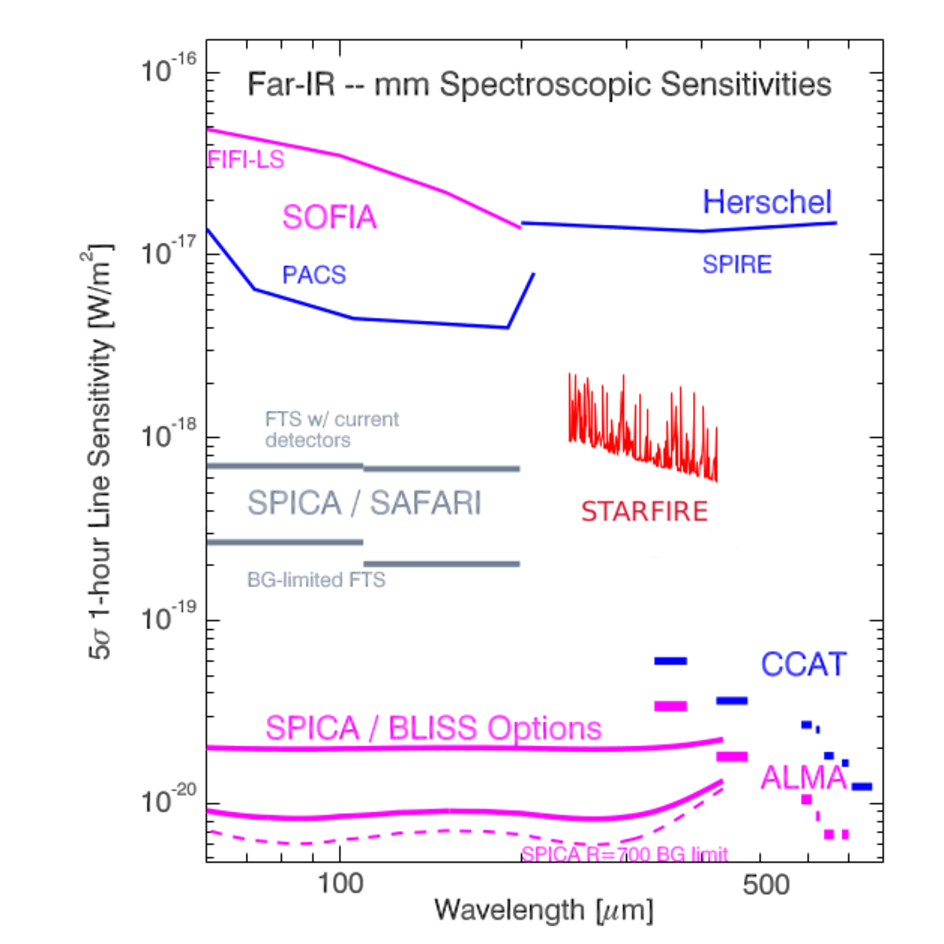
\includegraphics[height=3in]{sensitivity_2012.pdf}
      \end{center}
    \end{minipage} &
    \begin{minipage}{3.25in}
      \begin{center}
	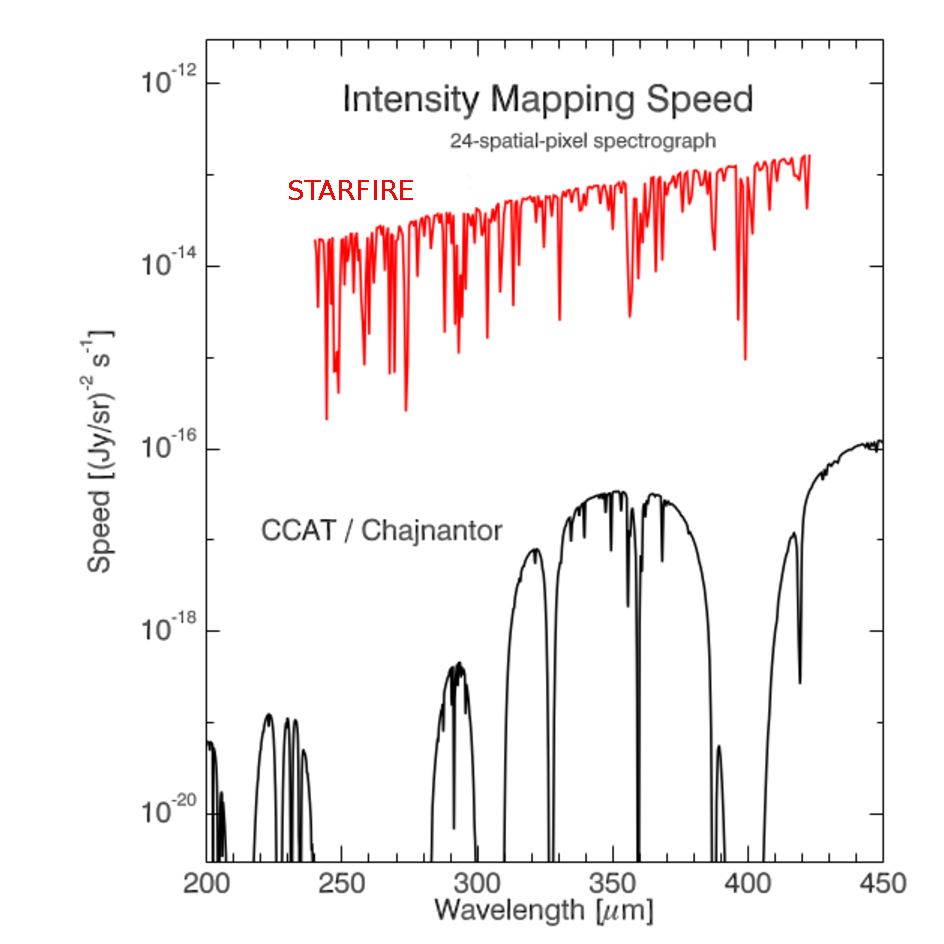
\includegraphics[height=3in]{icaris_nei.pdf}
      \end{center}
    \end{minipage}
  \end{tabular}
      \captionbaseline\caption{\small \L\ \name\ (red) compared to current and
	future spectroscopic instruments.  We compute a $5\sigma$ 1
	hour sensitivity on a single source as the benchmark. The
	variation in the \name\ sensitivity is due to atmospheric
	emission lines.  Approximately 10\% of the band is compromised
	due to these lines, though they may still be used for
	frequency calibration. \R\ The mapping speed of \name\
	compared to an identical instrument on CCAT.  Here larger
	values correspond to more area mapped to the same depth in the
	same time; a balloon instrument like \name\ is as much as 3 orders of magnitude
	faster.  Note that for intensity mapping, telescope area is
	not a factor.  Note also the significant regions in redshift
	not accessible from the ground even at the best sites.}
      \label{fig:SensCompare}
\end{figure}

%\clearpage




















